\begin{figure*}[t]
\centering
% src: fig/abc_locres.png by scripts/paper_figures_abc.py (render --paper); numbers: docs/paper/fig_abc_provenance.json (local_resolution); docs/paper/fig_abc_locres.csv
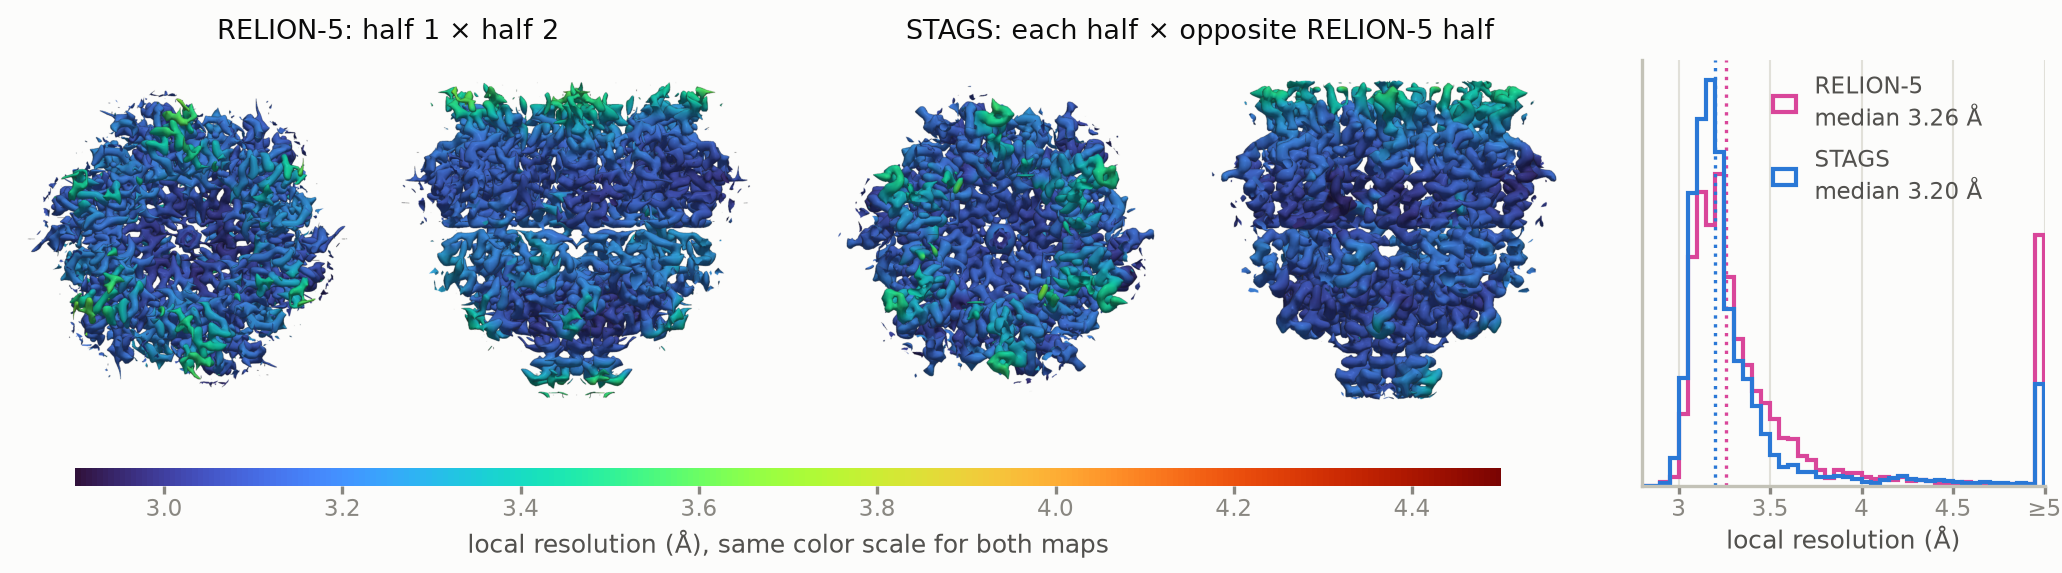
\includegraphics[width=\textwidth]{fig/abc_locres.png}
\caption{\textbf{Local resolution with one estimator for both maps.}
Top and side views of the central hexamer (surfaces as in the supplementary \cref{fig:views}), colored on one scale by windowed FSC~0.143 (40\,px box, cosine sphere from 10.8 to 18.9\,\AA, every 3\,px, phase-randomization correction beyond 20\,\AA); right, the distribution over all window centers inside RELION's mask.
RELION-5: its half 1 against half 2 (median 3.26\,\AA).
STAGS: each half against the opposite RELION-5 half (median 3.20\,\AA), which measures agreement with RELION, because STAGS's own half maps stay above FSC~0.143 up to Nyquist.}
\label{fig:locres}
\end{figure*}
